%% LyX 1.6.2 created this file.  For more info, see http://www.lyx.org/.
%% Do not edit unless you really know what you are doing.
\documentclass[english]{article}
\usepackage[T1]{fontenc}
\usepackage[latin1]{inputenc}
\setcounter{secnumdepth}{2}
\setcounter{tocdepth}{2}
\usepackage{verbatim}
\usepackage{graphicx}

%%%%%%%%%%%%%%%%%%%%%%%%%%%%%% Textclass specific LaTeX commands.
\newenvironment{lyxlist}[1]
{\begin{list}{}
{\settowidth{\labelwidth}{#1}
 \setlength{\leftmargin}{\labelwidth}
 \addtolength{\leftmargin}{\labelsep}
 \renewcommand{\makelabel}[1]{##1\hfil}}}
{\end{list}}
\newenvironment{lyxcode}
{\par\begin{list}{}{
\setlength{\rightmargin}{\leftmargin}
\setlength{\listparindent}{0pt}% needed for AMS classes
\raggedright
\setlength{\itemsep}{0pt}
\setlength{\parsep}{0pt}
\normalfont\ttfamily}%
 \item[]}
{\end{list}}

%%%%%%%%%%%%%%%%%%%%%%%%%%%%%% User specified LaTeX commands.
\makeatother

\usepackage{babel}

\begin{document}

\title{MAPI functions tutorial}

\maketitle

\section{Introduction}

This is a tutorial that shows how to implement new functions in MAPI.
It starts by giving detailed description of all structures and interfaces
that can be used by functions. It then shows several examples on how
some of the functions in the standard library is implemented, starting
with a simple function like PKT\_COUNTER and gradually moving towards
more advanced functions.


\section{Structures}

This is an overview of the structures that are used by MAPI functions.
Figure \ref{cap:Structure-relations} shows how the various structures
are connected.

%
\begin{figure}
\begin{centering}
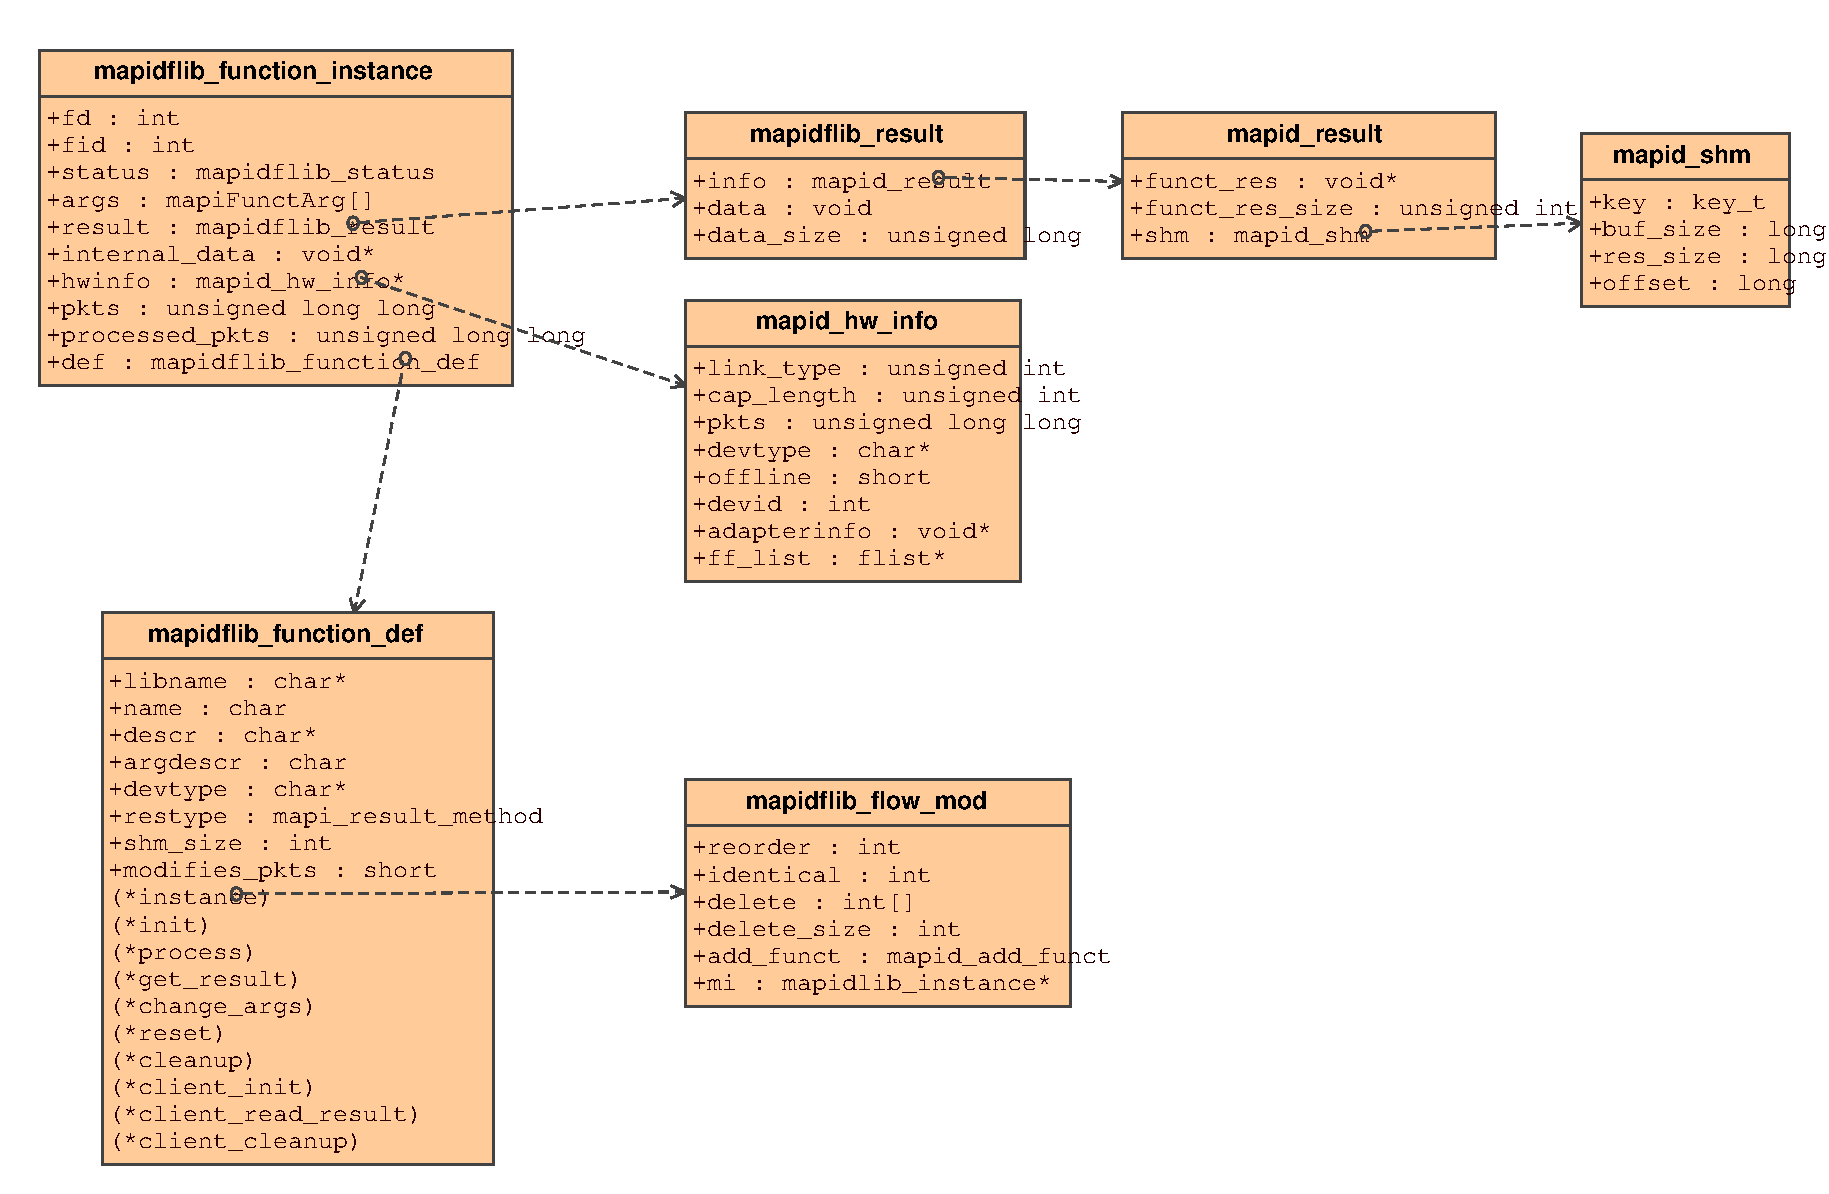
\includegraphics[width=1\linewidth,angle=90]{structures}
\par\end{centering}

\caption{\label{cap:Structure-relations}Structure relations.
Warning: contains outdated info, not accurate.}

\end{figure}



\subsection{\label{sub:mapidflib_function_def}mapidflib\_function\_def}

The mapidflib\_function\_def structure defines the static properties
of a function and has the following entries:
\begin{lyxlist}{00.00.0000}
\item [{char{*}~libname}] name of library that the function is part of. 
\item [{char{*}~name}] name of the function 
\item [{char{*}~descr}] description of the function 
\item [{char{*}~argdescr}] description of the arguments that a function
needs. Each character in the string specifies the type of an argument.
The following types are supported:

\begin{lyxlist}{00.00.0000}
\item [{s}] string 
\item [{i}] integer 
\item [{c}] single character 
\item [{l}] unsigned long long %\item [u]UID of the application
%\item [p]path of where the application is running

\item [{w}] filename for writing 
\item [{r}] reference to a flow 
\item [{f}] reference to a function 
\end{lyxlist}
A function that takes two integers and a string as arguments, will
then set argdescr to {}``iis''

\item [{char{*}~devtype}] specifies the type of device that this function
is compatible with. Valid device types are specified in the file \emph{mapidevices.h}. 
\item [{mapi\_result\_method\_t~restype}] specifies which method that
should be used for returning results to the client application. Valid
options are:

\begin{lyxlist}{00.00.0000}
\item [{MAPIRES\_NONE}] the function do not return any results 
\item [{MAPIRES\_IPC}] socket based IPC is used every time a result is
sent from the MAPI daemon to the client application. 
\item [{MAPIRES\_SHM}] results are returned using shared memory. 
\item [{MAPIRES\_FUNCT}] function specific method. The function must implement
its own method for returning results. 
\end{lyxlist}
\item [{int~shm\_size}] size of the shared memory in bytes.
Should be 0 if shm is not used.
\item [{short~modifies\_pkts}] if the function modifies packets this should
be set to 1. Support for functions that modifies packets is optional.
If a function that modifies packets is applied to a flow in a MAPI
system where support for it is turned off, an error message will be
returned to the user application. 
\item [{short~filters\_pkts}] if the function filters packets this should
be set to 1. This means that if the function lets all packets pass this
should be set to 0.
\item [{mapidfilb\_optimize\_t~optimize}] Method used for global optimization.
Options are:
\begin{lyxlist}{00.00.0000}
\item [{MAPIOPT\_NONE}] No global optimization should be used.
\item [{MAPIOPT\_AUTO}] Automatic global optimization.
\item [{MAPIOPT\_MANUAL}] Manual global optimization. Functions using this method
should  use the \emph{identical} field in the \emph{mapidflib\_flow\_mod}
structure for global optimization.
\end{lyxlist}
\item [{instance}] pointer to the instance interface of the function. See
section \ref{sub:instance} for details. 
\item [{init}] pointer to the init interface of the function. See section
\ref{sub:init} for details. 
\item [{process}] pointer to the processing interface of the function.
See section \ref{sub:process} for details. 
\item [{get\_result}] pointer to the get\_result interface. See section
\ref{sub:get_result} for details. 
\item [{reset}] pointer to the reset interface. See section \ref{sub:reset}
for details. 
\item [{cleanup}] pointer to the cleanup interface. See section \ref{sub:cleanup}
for details. 
\item [{client\_init}] pointer to the client\_init interface. See section
\ref{sub:client_init} for details. 
\item [{client\_read\_result}] pointer to the client\_read\_result interface.
See section \ref{sub:client_read_result} for details. 
\item [{client\_cleanup}] pointer to the client\_cleanup interface. See
section \ref{sub:client_cleanup} for details. 
\end{lyxlist}

\subsection{\label{sub:mapidflib_function_t}mapidflib\_function\_t}
The \emph{mapidflib\_function\_t} structure defines an applied function
and points to the function instance. Can be globally optimized to point
to a previously applied function instance.

\begin{lyxlist}{00.00.0000}
\item [{int~fd}] flow descriptor of the flow that the function belongs to. 
\item [{int~fid}] unique ID of the function 
\item [{int~ref}] is 1 if the reference is to an instance in other flow.
\item [{mapidflib\_function\_instance\_t~{*}instance}] pointer to the function
instance for this function. See section \ref{sub:mapidflib_function_instance}
for details.
\end{lyxlist}

\subsection{\label{sub:mapidflib_function_instance}mapidflib\_function\_instance}

The \emph{mapidflib\_function\_instance} structure defines the dynamic
properties of a running function.
\begin{lyxlist}{00.00.0000}
\item [{mapidflib\_status\_t~status}] current status of the function.
Valid values are:

\begin{lyxlist}{00.00.0000}
\item [{MAPIFUNC\_UNINIT}] the function is uninitialized 
\item [{MAPIFUNC\_INIT}] the function has been initialized 
\end{lyxlist}
\item [{{mapiFunctArg{[}{]}}~args}] arguments that were passed to the
function 
\item [{mapidflib\_result\_t~result}] structure that contains the results
of the function. See section \ref{sub:mapidflib_result} for more
details. 
\item [{void{*}~internal\_data}] pointer to internal data. The function
is free to use this as it wants. 
\item [{mapid\_hw\_info\_t~{*}hwinfo}] pointer to hardware specific information
about the adapter the function is running on. See section \ref{sub:mapid_hw_info}
for details. 
\item [{unsigned~long~long~pkts}] number of packets that has been sent
to the function. 
\item [{unsigned~long~long~processed\_pkts}] number of packets that
has been processed by the function and passed on to the next. 
\item [{mapidflib\_function\_def\_t~{*}def}] pointer to a copy of the
function definition. Since this is a copy, the definition can be changed
by the function during the initialization. 
\item [{int~ret}] return value of the last time the function proceesed
a packet.
\item [{int~refcount}] number of flows that references this function isntance.
\item [{int~apply\_flags}] copy of the flags argument from mapid\_apply\_function()
\end{lyxlist}

\subsection{\label{sub:mapidflib_result}mapidflib\_result}

The mapidflib\_result structure contains information about the results
of a function.
\begin{lyxlist}{00.00.0000}
\item [{mapid\_result\_t~info}] information about results that are sent
to the client. 
\item [{void~{*}data}] pointer to memory that contains the results. Functions
that needs access to results from other functions, uses this pointer
to read the results. 
\item [{unsigned~long~data\_size}] size of the result data. 
\end{lyxlist}

\subsection{\label{sub:mapid_result}mapid\_result}

Contains information about MAPI function results that is sent back
to the client.
\begin{lyxlist}{00.00.0000}
\item [{void~{*}funct\_res}] pointer to function specific information 
\item [{unsigned~fuct\_res\_size}] size of the function specific information 
\item [{mapid\_shm\_t~shm}] contains information about shared memory.
Functions should normally not need to access this structure themselves
as it is handled automatically by code in mapidlib.
\item [{mapid\_shm\_t~shm\_spinlock}] read/write spinlock for shared memory.
\end{lyxlist}

\subsection{\label{sub:mapid_hw_info}mapid\_hw\_info}

This structure contains information about a hardware adapter.
\begin{lyxlist}{00.00.0000}
\item [{unsigned~int~link\_type}] the link type of the adapter. 
\item [{unsigned~int~cap\_length}] the maximum length of a packet that
can be captured by the adapter 
\item [{unsigned~long~long~pkts}] number of packets captured by the
adapter 
\item [{unsigned~long~pkt\_drop}] numberof packets dropped by the hardware.
\item [{char~{*}devtype}] type of device as defined in mapidevices.h 
\item [{short~offline}] a value of 1 or more indicates that the device is used
for analyzing already captured trace files. 0 means proper online device.
\item [{int~devid}] unique ID of the adapter 
\item [{int~devfd}] file descriptor for hardware device
\item [{global\_function\_list\_t~{*}gflist}] global list of flows and the
functions applied to them. (gflist->fflist) There can be multiple flows
pointing to the same function, see \emph{optimize} field in section
\ref{sub:mapidflib_function_def} for details.
\item [{void~{*}adapterinfo}] adapter specific information 
\end{lyxlist}

\subsection{\label{sub:mapidflib_flow_mod}mapidflib\_flow\_mod}

This structure contains various variables that can be used by a function
to modify the behavior of a flow.
\begin{lyxlist}{00.00.0000}
\item [{int~reorder}] used for reordering the execution order of functions
in the flow. A function can set this to indicate that this function
should be processed before the function that has a function ID equal
to the the value of reorder. 
\item [{int~identical}] a function can check already applied functions
from the ff\_list in the hw\_info structure. If it finds an identical
function it can set this variable to point to it. The internal functions
in MAPId can then use this information to do global optimization. 
\item [{int~{*}delete}] pointer to a list of function IDs that can be
deleted. This can for example be used by a function if one instance
of this function can replace already applied functions. 
\item [{int~delete\_size}] number of entries in the delete array. 
\item [{mapid\_add\_function~add\_funct}] pointer to a function that can
be used for adding new functions to the flow. 
\item [{mapidlib\_instance\_t~{*}mi}] pointer to the mapidlib instance.
Used as an argument to mapid\_add\_function. 
\end{lyxlist}

\subsection{\label{sub:mapid_pkthdr}mapid\_pkthdr}

This structure contains information about a packet captured by a MAPI
driver.
\begin{lyxlist}{00.00.0000}
\item [{unsigned~long~long~ts}] 64-bit timestamp of packet. 
\item [{unsigned~short~ifindex}] interface index identifying which interface
on the adapter that was used to capture the packet. 
\item [{unsigned~caplen}] the number of bytes that was captured 
\item [{unsigned~wlen}] the actual length of the packet including link
layer header 
\item [{int~color}] colorization of the packet for optimizations
\end{lyxlist}

\section{MAPI function interfaces}

This is a description of the various interfaces that can be implemented
by a MAPI function. Many of the interfaces are optional.


\subsection{\label{sub:instance}instance}
\begin{lyxcode}
{\footnotesize int~instance(mapidflib\_function\_instance\_t~{*}instance,}{\footnotesize \par}

~{\footnotesize{}~~~~~~~~~~~~int~{*}fd,}{\footnotesize \par}

~{\footnotesize{}~~~~~~~~~~~~mapidflib\_flow\_mod\_t~{*}flow\_mod);}~
\end{lyxcode}
The instance interface is called when an application uses \emph{mapi\_apply\_function.}
This interface should do a syntax check of arguments that are passed
to the function. The function can also use this interface to indicate
similar functions, apply new functions or delete functions. No resources
should be allocated in this interface.


\subsubsection{Arguments}
\begin{lyxlist}{00.00.0000}
\item [{mapidflib\_function\_instance\_t~{*}instance}] pointer to the
instance of the function. See section \ref{sub:mapidflib_function_instance} 
\item [{int~{*}fd}] flow descriptior of the flow.
\item [{mapidflib\_flow\_mod\_t~{*}flow\_mod}] pointer to the structure
used for modifying the flow. See section \ref{sub:mapidflib_flow_mod}. 
\end{lyxlist}

\subsection{\label{sub:init}init}
\begin{lyxcode}
{\footnotesize int~init(mapidflib\_function\_instance\_t{*}~instance,~}{\footnotesize \par}

~{\footnotesize{}~~~~~~~~int~fd);}{\footnotesize \par}
\end{lyxcode}
The init interface is called when an application uses \emph{mapi\_connect}.
This interface allocates and initializes resources needed by the function.


\subsubsection{Arguments}
\begin{lyxlist}{00.00.0000}
\item [{mapidflib\_function\_instance\_t~{*}instance}] pointer to the
instance of the function. See section \ref{sub:mapidflib_function_instance} 
\item [{int~fd}] flow descriptior of the flow. 
\end{lyxlist}

\subsection{\label{sub:process}process}
\begin{lyxcode}
{\footnotesize int~process(mapidflib\_function\_instance\_t{*}~instance,}{\footnotesize \par}

~{\footnotesize{}~~~~~~~~~~~unsigned~char{*}~dev\_pkt,~}{\footnotesize \par}

~{\footnotesize{}~~~~~~~~~~~unsigned~char{*}~link\_pkt,}{\footnotesize \par}

~{\footnotesize{}~~~~~~~~~~~mapid\_pkthdr\_t{*}~pkt\_head);~}{\footnotesize \par}
\end{lyxcode}
This is the interface where the actual processing of a packet takes
place. If the function returns the value 1, then the next function
applied to the MAPI flow will be called. The value 0 means that further
processing of this flow should stop.


\subsubsection{Arguments}
\begin{lyxlist}{00.00.0000}
\item [{mapidflib\_function\_instance\_t~{*}instance}] pointer to the
instance of the function. See section \ref{sub:mapidflib_function_instance} 
\item [{unsigned~char~{*}dev\_pkt}] pointer to the packet as captured
by the device. This includes any device specific header. 
\item [{unsigned~char~{*}link\_pkt}] pointer to the packet starting at
the link layer header. 
\item [{mapid\_pkthdr\_t~{*}pkt\_head}] pointer to the packet header structure.
See section \ref{sub:mapid_pkthdr}. 
\end{lyxlist}

\subsection{\label{sub:get_result}get\_result}
\begin{lyxcode}
{\footnotesize int~get\_result(mapidflib\_function\_instance\_t{*}~instance,~~~~~~~~~~~~~~~~~~}{\footnotesize \par}

~{\footnotesize{}~~~~~~~~~~~~~~mapidflib\_result\_t~{*}{*}res);}{\footnotesize \par}
\end{lyxcode}
This interface returns the results of this function to other functions
or to the client application. MAPId has built in support for returning
results through IPC or shared memory. This interface is only needed
if these built in methods are not enough, for example if synchronization
between MAPId and the client is needed or if results are read directly
from the hardware adapter.


\subsubsection{Arguments}
\begin{lyxlist}{00.00.0000}
\item [{mapidflib\_function\_instance\_t~{*}instance}] pointer to the
instance of the function. See section \ref{sub:mapidflib_function_instance}. 
\item [{mapidflib\_result\_t~{*}{*}res}] pointer to the result structure
that is used for returning information needed by others to get hold
of the results. See section \ref{sub:mapid_result}. 
\end{lyxlist}


\subsection{\label{sub:reset}reset}
\begin{lyxcode}
{\footnotesize int~reset(mapidflib\_function\_instance\_t{*}~instance);}{\footnotesize \par}
\end{lyxcode}
This interface is called by other functions and is used for resetting
the results of the function.


\subsubsection{Arguments}
\begin{lyxlist}{00.00.0000}
\item [{mapidflib\_function\_instance\_t~{*}instance}] pointer to the
instance of the function. See section \ref{sub:mapidflib_function_instance} 
\end{lyxlist}

\subsection{\label{sub:cleanup}cleanup}
\begin{lyxcode}
{\footnotesize int~cleanup(mapidflib\_function\_instance\_t{*}~instance);}{\footnotesize \par}
\end{lyxcode}
This interface that is called when a flow is closed and should release
all allocated resources.


\subsubsection{Arguments}
\begin{lyxlist}{00.00.0000}
\item [{mapidflib\_function\_instance\_t~{*}instance}] pointer to the
instance of the function. See section \ref{sub:mapidflib_function_instance} 
\end{lyxlist}

\subsection{\label{sub:client_init}client\_init}
\begin{lyxcode}
{\footnotesize int~client\_init(mapidflib\_function\_instance\_t~{*}instance,~~~~~~~~~~~~~~~~~~}{\footnotesize \par}

~{\footnotesize{}~~~~~~~~~~~~~~~void{*}~data);}{\footnotesize \par}
\end{lyxcode}
This interface runs on the client side and is called the first time
\emph{mapi\_read\_results} is called. It is used for initializing
function specific code that runs on the client side.


\subsubsection{Arguments}
\begin{lyxlist}{00.00.0000}
\item [{mapidflib\_function\_instance\_t~{*}instance}] pointer to the
instance of the function. See section \ref{sub:mapidflib_function_instance} 
\item [{void~{*}data}] pointer to the function specific data that was
returned by the get\_result interface. 
\end{lyxlist}

\subsection{\label{sub:client_read_result}client\_read\_result}
\begin{lyxcode}
{\footnotesize int~client\_read\_result(mapidflib\_function\_instance\_t{*}~instance,~}{\footnotesize \par}

~{\footnotesize{}~~~~~~~~~~~~~~~~~~~~~~mapi\_result\_t~{*}res);}{\footnotesize \par}
\end{lyxcode}
This interface is called each time \emph{mapi\_read\_results} is used.
It runs on the client side and is used for implementing function specific
methods for returning results to the user application.


\subsubsection{Arguments}
\begin{lyxlist}{00.00.0000}
\item [{mapidflib\_function\_instance\_t~{*}instance}] pointer to the
instance of the function. See section \ref{sub:mapidflib_function_instance} 
\item [{mapi\_result\_t~{*}res}] pointer to the result structure. See
section \ref{sub:mapid_result}. 
\end{lyxlist}

\subsection{\label{sub:client_cleanup}client\_cleanup}
\begin{lyxcode}
{\footnotesize int~client\_cleanup(mapidflib\_function\_instance\_t{*}~instance);}{\footnotesize \par}
\end{lyxcode}
This interface is called when the flow closes and should release all
resources allocated by the function on the client side.


\subsubsection{Arguments}
\begin{lyxlist}{00.00.0000}
\item [{mapidflib\_function\_instance\_t~{*}instance}] pointer to the
instance of the function. See section \ref{sub:mapidflib_function_instance} 
\end{lyxlist}

\section{Tutorials}

In this section we will demonstrate how to create new MAPI functions
through a series of tutorials. All the functions are taken from the
standard library, but during the tutorials we will create a new library,
\emph{tutlib}, to which we will add one function at the time.

When there exists two functions with the same name and for the same
device type, the first one found will be used. To make sure that functions
from the new library is chosen, one must specify the name of the library
in the mapi\_apply\_function call like this:
\begin{lyxcode}
{\footnotesize mapi\_apply\_function(fd,''tutlib:<function~name>'')}{\footnotesize \par}
\end{lyxcode}

\subsection{Simple function: PKT\_COUNTER}

The first function we will create is a simple packet counter. All
this function does is to increment a counter each time the process
interface is called. Results are sent to the client using shared memory.


\subsubsection{Implementation}

To start off we first have to create a new directory for the new library.
In the main mapi directory do:
\begin{lyxcode}
{\footnotesize mkdir~tutlib}{\footnotesize \par}

{\footnotesize cd~tutlib}{\footnotesize \par}
\end{lyxcode}
To create the new function we can use the function template located
in the mapi main directory:
\begin{lyxcode}
{\footnotesize cp~../funct\_template.c~pktcounter.c}{\footnotesize \par}
\end{lyxcode}
In this template all the MAPI function interfaces are present. Most
of these are not needed for the simple packet counter functions so
the first thing to do is to remove them. For this function only process
and reset are needed.

We will use the prefix \emph{pktc} for each function in the source
code, so we should replace the text \emph{<funct\_name>} with pktc.
We are then left with only two interfaces like this:
\begin{lyxcode}
{\footnotesize static~int~pktc\_process(mapidflib\_function\_instance\_t~{*}instance,~~~~~~~~~~~~~~~~~~~~~~~~~~}{\footnotesize \par}

~{\footnotesize{}~~~~~~~~~~~~~~~~~~~~~~~const~unsigned~char{*}~dev\_pkt,~~~~~~~~~~~~~~~~~~~~~~~~~~~~~}{\footnotesize \par}

~{\footnotesize{}~~~~~~~~~~~~~~~~~~~~~~~const~unsigned~char{*}~link\_pkt,~~~~~~~~~}{\footnotesize \par}

~{\footnotesize{}~~~~~~~~~~~~~~~~~~~~~~~mapid\_pkthdr\_t{*}~pkt\_head)~~~}{\footnotesize \par}

{\footnotesize \{~~~}{\footnotesize \par}

~{\footnotesize{}~return~1;~}{\footnotesize \par}

{\footnotesize \}}{\footnotesize \par}

{\footnotesize static~int~pktc\_reset(mapidflib\_function\_instance\_t~{*}instance)~~}{\footnotesize \par}

{\footnotesize \{~~~}{\footnotesize \par}

~{\footnotesize{}~return~0;~}{\footnotesize \par}

{\footnotesize \}}{\footnotesize \par}
\end{lyxcode}
We can now move on to the mapidflib\_function\_def structure that
defines the function. The entries in this structure should be modified
like this:
\begin{lyxlist}{00.00.0000}
\item [{libname}] empty string. This is set by the library that includes
the function 
\item [{name}] The function name can be set to any value but in this example
we will call the function PKT\_COUNTER 
\item [{descr}] free text describing the function. 
\item [{argdescr}] the function do not take any arguments so this should
be an empty string. 
\item [{devtype}] we will implement a generic software function that runs
on top of all adapters. The devtype should therefor be set to \emph{MAPI\_DEVICE\_ALL}. 
\item [{restype}] results are returned by shared memory so this should
be set to \emph{MAPIRES\_SHM}. 
\item [{shm\_size}] the function returns an unsigned long long counter
so this should be set to \emph{sizeof(unsigned long long)} 
\item [{modifies\_pkts}] the function do not modify any packets so this
should be set to \emph{0} 
\item [{filters\_pkts}] the function do not filter any packets so this
is also set to \emph{0}
\item [{optimize}] the function will not use global optimization. So
we set this to \emph{MAPIOPT\_NONE}.
\item [{process}] should be set to the address of the pktc\_process interface 
\item [{reset}] should be set to the address of the pktc\_reset interface 
\end{lyxlist}
For the rest of the MAPI function interfaces in the structure, the
value should be set to \emph{NULL} since these functions do not exist.

With these modifications we get a structure looking like this:
\begin{lyxcode}
{\footnotesize static~mapidflib\_function\_def\_t~finfo=\{}{\footnotesize \par}

~{\footnotesize{}~\textquotedbl{}\textquotedbl{},~//libname~~~}{\footnotesize \par}

~{\footnotesize{}~\textquotedbl{}PKT\_COUNTER\textquotedbl{},~//name~~~}{\footnotesize \par}

~{\footnotesize{}~\textquotedbl{}Counts~number~of~packets\textbackslash{}n\textbackslash{}tReturn~value:~unsigned~long~long\textquotedbl{},~//descr~~~}{\footnotesize \par}

~{\footnotesize{}~\textquotedbl{}\textquotedbl{},~//argdescr~~~}{\footnotesize \par}

~{\footnotesize{}~MAPI\_DEVICE\_ALL,~//devtype~~~}{\footnotesize \par}

~{\footnotesize{}~MAPIRES\_SHM,~//Method~for~returning~results~~~}{\footnotesize \par}

~{\footnotesize{}~sizeof(unsigned~long~long),~//shm~size~~~}{\footnotesize \par}

~{\footnotesize{}~0,~//modifies\_pkts~~~}{\footnotesize \par}

~{\footnotesize{}~0,~//filters\_pkts~~~}{\footnotesize \par}

~{\footnotesize{}~MAPIOPT\_NONE,~//optimize~~~}{\footnotesize \par}

~{\footnotesize{}~NULL,~//instance~~~}{\footnotesize \par}

~{\footnotesize{}~NULL,~//init~~~}{\footnotesize \par}

~{\footnotesize{}~pktc\_process,~//process~~~}{\footnotesize \par}

~{\footnotesize{}~NULL,~//get\_result,~~~}{\footnotesize \par}

~{\footnotesize{}~pktc\_reset,~//reset~~~}{\footnotesize \par}

~{\footnotesize{}~NULL,~//cleanup~~~}{\footnotesize \par}

~{\footnotesize{}~NULL,~//client\_init~~~}{\footnotesize \par}

~{\footnotesize{}~NULL,~//client\_read\_result~~~}{\footnotesize \par}

~{\footnotesize{}~NULL~~//client\_cleanup~}{\footnotesize \par}

{\footnotesize \};}{\footnotesize \par}
\end{lyxcode}
At the end of the file there is also a function called get\_funct\_info.
This is used by the library to return information from the function.
The only change necessary for this function is to change the <funct\_name>
to \emph{pktc} so that the full name of the function becomes pktc\_funct\_info.

We can now start to look at the actual code for this packet counter
MAPI function. Since we use shared memory, allocation and initializing
the memory to 0 is already taken care of. In the processing interface
all that is needed is to increment the unsigned long long counter
in the shared memory. The location of this counter is pointed to by
the data pointer in the result structure of the current instance.
The code inside the pktc\_process interface should then simply be:
\begin{lyxcode}
~({*}(unsigned~long~long{*})instance->result.data)++;
\end{lyxcode}
The code for the rest interface is similar and just reset the shared
memory counter to zero:
\begin{lyxcode}
~({*}(unsigned~long~long{*})instance->result.data)=0;
\end{lyxcode}
The entire source code for the packet counter function should then
be:

{\footnotesize \verbatiminput{tutlib/pktcounter.c}}{\footnotesize \par}


\subsubsection{Function library}

To be able to use this new MAPI function from an application, it must
be included in a library. For this tutorial we will create a new library,
tutlib, by using createlib.pl:
\begin{lyxcode}
../createlib.pl~tutlib~tutlib.c
\end{lyxcode}
This will create a new library called \emph{tutlib} in the file \emph{tutlib.c}.
All functions in the current directory will automatically be included
in the library.


\subsubsection{Makefile}

We can now compile the new function and library. To do this it is
best to create a Makefile. The contents of a makefile could look like
this:
\begin{lyxcode}
{\footnotesize INCLUDE=-I.~-I..}{\footnotesize \par}

{\footnotesize CFLAGS=-g~-Wall~-Wsign-compare~-Wpointer-arith~-Wnested-externs~\textbackslash{}~}{\footnotesize \par}

~{\footnotesize{}~~~~~~-Wmissing-declarations~-Wcast-align~-D\_GNU\_SOURCE~\$(INCLUDE)~\textbackslash{}}{\footnotesize \par}

~~~~~-DDEBUG=1

{\footnotesize TARGETS=tutlib.so}{\footnotesize \par}

{\footnotesize all:~\$(TARGETS)}{\footnotesize \par}

{\footnotesize tutlib.o:~tutlib.c~../mapidflib.h~../mapi.h~~~~~}{\footnotesize \par}

~{\footnotesize{}~gcc~\$(CFLAGS)~-c~\$<}{\footnotesize \par}

{\footnotesize tutlib.so:~tutlib.o~pktcounter.o}{\footnotesize \par}

~{\footnotesize{}~gcc~\$(CFLAGS)~-shared~~-o~\$@~\$\textasciicircum{}~-lfl~-lrt~-L..~-L.~\$(LIB\_DIR)}{\footnotesize \par}

{\footnotesize pktcounter.o:~pktcounter.c~~~~~~}{\footnotesize \par}

~{\footnotesize{}~gcc~\$(CFLAGS)~-c~\$<}{\footnotesize \par}

{\footnotesize clean:~~}{\footnotesize \par}

~{\footnotesize{}~@/bin/rm~-f~{*}.o~{*}.so~{*}\textasciitilde{}~\$(TARGETS)}{\footnotesize \par}
\end{lyxcode}
The new MAPI function and library can now be compiled by running make.
The last step to be able to use the new function is to make sure that
the tutlib library is loaded when MAPId is started. To do this modify
mapi.conf so that the \emph{libpath} entry includes the tutlib directory
and the the \emph{libs} entry includes the tutlib library. It should
look something like this:
\begin{lyxcode}
{\footnotesize libpath=.:ipfixlib:tutlib}{\footnotesize \par}

{\footnotesize libs=mapidstdflib.so:ipfixlib.so:tutlib.so}{\footnotesize \par}
\end{lyxcode}

\subsection{Function with internal data: GAP}

This is a slightly more advanced function that uses internal data
to store information between each call to the process interface. The
function calculates the gap or the time that has elapsed between to
consecutive packets in a flow.


\subsubsection{Implementation}

Go to the tutlib directory created in the previous section. Copy the
function template:
\begin{lyxcode}
{\footnotesize cp~../funct\_template.c~gap.c}{\footnotesize \par}
\end{lyxcode}
Interfaces that are not needed should be removed. Since this function
uses internal data, the init and cleanup interfaces are needed in
addition to the process interface. The string \emph{<funct\_name>}
should be replaced with \emph{gap} and the mapidflib\_function\_def
structure needs modification so that it looks like:
\begin{lyxcode}
{\footnotesize static~mapidflib\_function\_def\_t~finfo=\{~~~}{\footnotesize \par}

~{\footnotesize{}~\textquotedbl{}\textquotedbl{},~//libname~~~}{\footnotesize \par}

~{\footnotesize{}~\textquotedbl{}GAP\textquotedbl{},~//name~~~}{\footnotesize \par}

~{\footnotesize{}~\textquotedbl{}Returns~the~gap~between~to~consecutive~packets\textbackslash{}n}{\footnotesize \par}

~{\footnotesize{}~~Return~value:~unsigned~long~long\textquotedbl{},~//descr~~~}{\footnotesize \par}

~{\footnotesize{}~\textquotedbl{}\textquotedbl{},~//argdescr~~~}{\footnotesize \par}

~{\footnotesize{}~MAPI\_DEVICE\_ALL,~//devoid~~~}{\footnotesize \par}

~{\footnotesize{}~MAPIRES\_SHM,~//Method~for~returning~results~~~}{\footnotesize \par}

~{\footnotesize{}~sizeof(unsigned~long~long),~//shm~size~~~}{\footnotesize \par}

~{\footnotesize{}~0,~//modifies\_pkts}{\footnotesize \par}

~{\footnotesize{}~0,~//filters\_pkts}{\footnotesize \par}

~{\footnotesize{}~MAPIOPT\_NONE,~//optimize}{\footnotesize \par}

~{\footnotesize{}~NULL,~//instance~~}{\footnotesize \par}

~{\footnotesize{}~gap\_init,~//~~~gap\_init,~~~}{\footnotesize \par}

~{\footnotesize{}~gap\_process,~~~}{\footnotesize \par}

~{\footnotesize{}~NULL,~//get\_result,~~~}{\footnotesize \par}

~{\footnotesize{}~NULL,~//reset~~~}{\footnotesize \par}

~{\footnotesize{}~gap\_cleanup,~//cleanup~~~}{\footnotesize \par}

~{\footnotesize{}~NULL,~//client\_init~~~}{\footnotesize \par}

~{\footnotesize{}~NULL,~//client\_read\_result~~~}{\footnotesize \par}

~{\footnotesize{}~NULL~~//client\_cleanup~}{\footnotesize \par}

{\footnotesize \};}{\footnotesize \par}
\end{lyxcode}
We are now ready to implement the code for the three interfaces this
MAPI function needs. What this function do is to store the time stamp
of a packet and when the next packet is captured it calculates the
time difference between the new and old timestamp. This means that
it needs to store the timestamp of a packet as internal data so that
it can be accessed again when the next packet is processed.

Timestamps are unsigned long long values so the init interface should
simply allocate memory to store such a value and let the internal\_data
pointer point to this memory. The function should also initialize
the unsigned long long value to 0. The code for this is then:
\begin{lyxcode}
{\footnotesize instance->internal\_data=malloc(sizeof(unsigned~long~long));~}{\footnotesize \par}

{\footnotesize {*}((unsigned~long~long{*})instance->internal\_data)=0;}{\footnotesize \par}
\end{lyxcode}
The process interface stores the difference between the timestamp
of the current packet and the previous one and stores it in the result
data:
\begin{lyxcode}
{\footnotesize unsigned~long~long~{*}gap,{*}old;~~~}{\footnotesize \par}

{\footnotesize old=instance->internal\_data;~~~}{\footnotesize \par}

{\footnotesize gap=instance->result.data;~~~~~~}{\footnotesize \par}

{\footnotesize if({*}old!=0)~~~~~}{\footnotesize \par}

~{\footnotesize{}~{*}gap=pkt\_head->ts-{*}old;~~~~~~}{\footnotesize \par}

{\footnotesize {*}old=pkt\_head->ts;}{\footnotesize \par}
\end{lyxcode}
When the flow closes, the internal data has to be freed. This is done
by the cleanup interface:
\begin{lyxcode}
{\footnotesize free(instance->internal\_data);}{\footnotesize \par}
\end{lyxcode}
The entire source code for this function would then be:

{\footnotesize \verbatiminput{tutlib/gap.c}}{\footnotesize \par}


\subsubsection{Function library}

The function library is recreated using the createlib.pl script as
in the previous section:
\begin{lyxcode}
{\footnotesize ../createlib.pl~tutlib~tutlib.c}{\footnotesize \par}
\end{lyxcode}

\subsubsection{Makefile}

The Makefile created in the previous section must be modified so that
it compiles the new function:
\begin{lyxcode}
{\footnotesize INCLUDE=-I.~-I..}{\footnotesize \par}

{\footnotesize CFLAGS=-g~-Wall~-Wsign-compare~-Wpointer-arith~-Wnested-externs~\textbackslash{}}{\footnotesize \par}

{\footnotesize -Wmissing-declarations~-Wcast-align~-D\_GNU\_SOURCE~\$(INCLUDE)}{\footnotesize \par}

{\footnotesize TARGETS=tutlib.so}{\footnotesize \par}

{\footnotesize all:~\$(TARGETS)}{\footnotesize \par}

{\footnotesize tutlib.o:~tutlib.c~../mapidflib.h~../mapi.h~~~~~}{\footnotesize \par}

~{\footnotesize{}~gcc~\$(CFLAGS)~-c~\$<}{\footnotesize \par}

{\footnotesize tutlib.so:~tutlib.o~pktcounter.o~gap.o}{\footnotesize \par}

~{\footnotesize{}~gcc~\$(CFLAGS)~-shared~~-o~\$@~\$\textasciicircum{}~-lfl~-lrt~-L..~-L.~\$(LIB\_DIR)}{\footnotesize \par}

~{\footnotesize{}~cp~\$@~..~}{\footnotesize \par}

{\footnotesize pktcounter.o:~pktcounter.c~~~~~~}{\footnotesize \par}

~{\footnotesize{}~gcc~\$(CFLAGS)~-c~\$<}{\footnotesize \par}

{\footnotesize gap.o:~gap.c~~~~~~}{\footnotesize \par}

~{\footnotesize{}~gcc~\$(CFLAGS)~-c~\$<}{\footnotesize \par}

{\footnotesize clean:~~}{\footnotesize \par}

~{\footnotesize{}~@/bin/rm~-f~{*}.o~{*}.so~{*}\textasciitilde{}~\$(TARGETS)}{\footnotesize \par}
\end{lyxcode}

\subsection{Function with multiple process interfaces: PKTINFO}

We are now going to implement a function that returns some information
about a packet. To keep things simple we will limit the information
to either packet length or timestamp. Results from this function will
typical be used by other functions for further processing.


\subsubsection{Implementation}

As in the previous examples, start by copying the function template
and set the function name to pktinfo:
\begin{lyxcode}
{\footnotesize cp~../funct\_template.c~pktinfo.c}{\footnotesize \par}
\end{lyxcode}
This function will need an argument to decide which information that
should be returned. This means that we need to specify the type of
argument in the mapidflib\_function\_def structure. We will also need
to implement the instance interface to do a syntax check of the argument.
The argument type will be an integer so the argdescr should be set
to {}``i''.

Since the information returned by the function is the same for the
entire lifetime of the function it is a waste of clock cycles to do
a check for every packet to decide which type of information should
be returned. Instead we can implement two version of the process interface,
one that returns packet length and one that returns the timestamp.
We can decide in the instance interface which process interface to
use.

The mapidflib\_function\_def structure should then look like this:
\begin{lyxcode}
{\footnotesize static~mapidflib\_function\_def\_t~finfo=\{~~~}{\footnotesize \par}

~{\footnotesize{}~\textquotedbl{}\textquotedbl{},~//libname~~~}{\footnotesize \par}

~{\footnotesize{}~\textquotedbl{}PKTINFO\textquotedbl{},~//name~~~}{\footnotesize \par}

~{\footnotesize{}~\textquotedbl{}Returns~information~about~a~packet~as~unsigned~long~long\textquotedbl{},~~~}{\footnotesize \par}

~{\footnotesize{}~\textquotedbl{}i\textquotedbl{},~//argdescr~~~}{\footnotesize \par}

~{\footnotesize{}~MAPI\_DEVICE\_ALL,~//devoid~~~}{\footnotesize \par}

~{\footnotesize{}~MAPIRES\_SHM,~//Method~for~returning~results~~~}{\footnotesize \par}

~{\footnotesize{}~sizeof(unsigned~long~long),~//shm~size~~~}{\footnotesize \par}

~{\footnotesize{}~0,~//modifies\_pkts~~~}{\footnotesize \par}

~{\footnotesize{}~0,~//filters\_pkts~~~}{\footnotesize \par}

~{\footnotesize{}~MAPIOPT\_NONE,~//optimize~~~}{\footnotesize \par}

~{\footnotesize{}~pktinfo\_instance,~~~}{\footnotesize \par}

~{\footnotesize{}~NULL,~//init~~~}{\footnotesize \par}

~{\footnotesize{}~NULL,~//process~~~}{\footnotesize \par}

~{\footnotesize{}~NULL,~//get\_result,~~~}{\footnotesize \par}

~{\footnotesize{}~NULL,~//reset~~~}{\footnotesize \par}

~{\footnotesize{}~NULL,~//cleanup~~~}{\footnotesize \par}

~{\footnotesize{}~NULL,~//client\_init~~~}{\footnotesize \par}

~{\footnotesize{}~NULL,~//client\_read\_result~~~}{\footnotesize \par}

~{\footnotesize{}~NULL~~//client\_cleanup~}{\footnotesize \par}

{\footnotesize \};}{\footnotesize \par}
\end{lyxcode}
To make things more user friendly we will first create an enum that
can be used for specifying the type of information that should be
returned by the function. This is placed in the file pktinfo.h:
\begin{lyxcode}
{\footnotesize \#ifndef~\_pktinfo\_h~}{\footnotesize \par}

{\footnotesize \#define~\_pktinfo\_h}{\footnotesize \par}

{\footnotesize enum~pktinfo~\{~~~PKT\_TS,PKT\_SIZE~\};}{\footnotesize \par}

{\footnotesize \#endif}{\footnotesize \par}
\end{lyxcode}
The code in the instance interface should then verify that the value
of the argument is either \emph{PKT\_TS} or \emph{PKT\_SIZE} . If
the value is not one of these, an error message should be returned.
Based on the argument the instance interface should then modify the
function instance copy of the mapidflib\_function\_def structure so
that the process pointer points to one of the two processing interfaces
that are implemented.

To implement the instance interface we should start by defining to
variables, one for storing the type of information that should be
returned and one pointer for pointing to the arguments:
\begin{lyxcode}
{\footnotesize int~type;~~~}{\footnotesize \par}

{\footnotesize mapiFunctArg{*}~fargs;}{\footnotesize \par}
\end{lyxcode}
To parse function arguments, the getarg functions found in mapiipc.h
can be used. To get hold of the integer that specifies the information
type we use:
\begin{lyxcode}
{\footnotesize fargs=instance->args;}{\footnotesize \par}

{\footnotesize type~=~getargint(\&fargs);}{\footnotesize \par}
\end{lyxcode}
We can now check the value of \emph{type} and set the pointer to the
correct process interface accordingly:
\begin{lyxcode}
{\footnotesize if(type==PKT\_SIZE)~~~~~~~}{\footnotesize \par}

~{\footnotesize{}~instance->def->process=pktinfo\_process\_size;~~~~~}{\footnotesize \par}

{\footnotesize else~if(type==PKT\_TS)~~~~~~~}{\footnotesize \par}

~{\footnotesize{}~instance->def->process=pktinfo\_process\_ts;~~~}{\footnotesize \par}

{\footnotesize else~~~~~}{\footnotesize \par}

~{\footnotesize{}~return~MFUNCT\_INVALID\_ARGUMENT\_2;}{\footnotesize \par}
\end{lyxcode}
The last step is to implement the two processing interfaces, \emph{pktinfo\_process\_size}
and \emph{pktinfo\_process\_ts.} The code for the interface returning
packet size will be:
\begin{lyxcode}
{\footnotesize ({*}(unsigned~long~long{*})instance->result.data)=}{\footnotesize \par}

~{\footnotesize{}~(unsigned~long~long)pkt\_head->wlen;~~~}{\footnotesize \par}

{\footnotesize return~1;}{\footnotesize \par}
\end{lyxcode}
For returning the packet timestamp we get:
\begin{lyxcode}
{\footnotesize ({*}(unsigned~long~long{*})instance->result.data)=}{\footnotesize \par}

~{\footnotesize{}~(unsigned~long~long)pkt\_head->ts;~~~}{\footnotesize \par}

{\footnotesize return~1;}{\footnotesize \par}
\end{lyxcode}
The entire code for the pktinfo function will then be:

{\footnotesize \verbatiminput{tutlib/pktinfo.c}}{\footnotesize \par}


\subsubsection{Function library and Makefile}

The function library and Makefile must be updated in the same way
as explained in the previous section.


\subsection{Function that reads results from other functions: STAT}

The statistical function reads unsigned long long values from other
functions and calculates the total number of values read, the sum,
square of sum, maximum and minimum values. It is a good example of
how one function can read results from another function.


\subsubsection{Implementation}

Copy the function template from the mapi main directory:
\begin{lyxcode}
{\footnotesize cp~../funct\_template.c~stat.c}{\footnotesize \par}
\end{lyxcode}
Replace the text {}``<funct\_name>'' with the text {}``stat''.
Delete interfaces that are not needed. This function needs arguments
and uses internal data to store information so it need to implement
the instance, init, process and cleanup interfaces.

The function will take three argument, one integer that specifies the
flow ID of the flow and one integer that specifies the function ID
of the function that the results should be read from and one char
that specifies if the result from the first packet should
be skipped. The last parameter is needed if we are reading results
from a function like GAP. This function will always return a 0 when
the very first packet is processed and if we did not skip this first
result, the minimum value would always become 0 in the STAT function.

This function will count the number of values read from another function,
the sum, square of sum, maximum and minimum value. All this information
will be stored in a structure placed in a stats.h file:
\begin{lyxcode}
{\footnotesize \#ifndef~\_STATS\_H~}{\footnotesize \par}

{\footnotesize \#define~\_STATS\_H~1}{\footnotesize \par}

{\footnotesize typedef~struct~stats~\{~~~}{\footnotesize \par}

~{\footnotesize{}~unsigned~long~long~count;~//Number~of~elements~~~}{\footnotesize \par}

~{\footnotesize{}~long~double~sum;~//Sum~~~}{\footnotesize \par}

~{\footnotesize{}~long~double~sum2;~//Sum~of~square~~~}{\footnotesize \par}

~{\footnotesize{}~double~max;~//Maximum~value~~~}{\footnotesize \par}

~{\footnotesize{}~double~min;~//Minimum~value~}{\footnotesize \par}

{\footnotesize \}~stats\_t;}{\footnotesize \par}

{\footnotesize \#endif}{\footnotesize \par}
\end{lyxcode}
It is also this structure that is returned to an application that
calls mapi\_read\_result.

The function will then need an instance interface for verifying the
arguments, an init interface to initialize internal resources that
stores the statistics, a processing interface to do the processing
of packets and a reset interface for resetting the results. The mapidflib\_function\_def
interface should then be:
\begin{lyxcode}
{\footnotesize static~mapidflib\_function\_def\_t~finfo=\{~~~}{\footnotesize \par}

~{\footnotesize{}~\textquotedbl{}\textquotedbl{},~//libname~~~}{\footnotesize \par}

~{\footnotesize{}~\textquotedbl{}STATS\textquotedbl{},~//name~~~}{\footnotesize \par}

~{\footnotesize{}~\textquotedbl{}Returns~statistical~information~about~}{\footnotesize \par}

~{\footnotesize{}~~unsigned~long~long~values~from~other~functions\textquotedbl{},}{\footnotesize \par}

~{\footnotesize{}~\textquotedbl{}iic\textquotedbl{},~//argdescr~~~}{\footnotesize \par}

~{\footnotesize{}~MAPI\_DEVICE\_ALL,~//devtype~~~}{\footnotesize \par}

~{\footnotesize{}~MAPIRES\_SHM,~//Method~for~returning~results~~~}{\footnotesize \par}

~{\footnotesize{}~sizeof(stats\_t),~//shm~size~~~}{\footnotesize \par}

~{\footnotesize{}~0,~//modifies\_pkts~~~}{\footnotesize \par}

~{\footnotesize{}~0,~//filters\_pkts~~~}{\footnotesize \par}

~{\footnotesize{}~MAPIOPT\_NONE,~//optimize~~~}{\footnotesize \par}

~{\footnotesize{}~stats\_instance,~//instance~~~}{\footnotesize \par}

~{\footnotesize{}~stats\_init,~//init~~~}{\footnotesize \par}

~{\footnotesize{}~stats\_process,~//process~~~}{\footnotesize \par}

~{\footnotesize{}~NULL,~//get\_result,~~~}{\footnotesize \par}

~{\footnotesize{}~stats\_reset,~//reset~~~}{\footnotesize \par}

~{\footnotesize{}~stats\_cleanup,~//cleanup~~~}{\footnotesize \par}

~{\footnotesize{}~NULL,~//client\_init~~~}{\footnotesize \par}

~{\footnotesize{}~NULL,~//client\_read\_result~~~}{\footnotesize \par}

~{\footnotesize{}~NULL~~//client\_cleanup~}{\footnotesize \par}

{\footnotesize \};~}{\footnotesize \par}
\end{lyxcode}
In the instance interface we must check that the first argument points
to an already existing function applied to the flow and we should
check that the third parameter is either a 0 or a 1. To get the values
of the arguments that is passed to the function getargint and
getargchar is used. To check the first two parameter we use a helper
function that loops through the flow list and then the function list
for the flow if it is found. The code would then be:
\begin{lyxcode}
{\footnotesize static~int~stats\_instance(mapidflib\_function\_instance\_t~{*}instance,~}{\footnotesize \par}

~{\footnotesize{}~~~~~~~~~~~~~~~~~~~~~~~~~int~fd,}{\footnotesize \par}

~{\footnotesize{}~~~~~~~~~~~~~~~~~~~~~~~~~mapidflib\_flow\_mod\_t~{*}flow\_mod)~}{\footnotesize \par}

{\footnotesize \{~~~}{\footnotesize \par}

~{\footnotesize{}~int~fid,afd;~~~}{\footnotesize \par}

~{\footnotesize{}~mapiFunctArg{*}~fargs;~~}{\footnotesize \par}

~{\footnotesize{}~int~skip;}{\footnotesize \par}

~{\footnotesize{}~}{\footnotesize \par}

~{\footnotesize{}~fargs=instance->args;}{\footnotesize \par}

~{\footnotesize{}~afd~=~getargint(\&fargs);~~~}{\footnotesize \par}

~{\footnotesize{}~fid~=~getargint(\&fargs);~~~}{\footnotesize \par}

~{\footnotesize{}~skip=getargchar(\&fargs);}{\footnotesize \par}

~

~{\footnotesize{}~if(fhlp\_get\_function\_instance(instance->hwinfo->gflist,afd,fid)==NULL)~~~~~}{\footnotesize \par}

~{\footnotesize{}~~~return~MFUNCT\_INVALID\_ARGUMENT\_1;}{\footnotesize \par}

~{\footnotesize{}~if(skip>1~||~skip<0)~~~~~~~}{\footnotesize \par}

~{\footnotesize{}~~~return~MFUNCT\_INVALID\_ARGUMENT\_2;~~~~~~~~}{\footnotesize \par}

~{\footnotesize{}~}{\footnotesize \par}

~{\footnotesize{}~return~0;~}{\footnotesize \par}

{\footnotesize \};}{\footnotesize \par}
\end{lyxcode}
In the init interface we have to store a reference to the function
which results are read from as well as the value for the skip argument
so that these can be used when processing packets. To do this we define
a structure that the internal\_data pointer can point to:
\begin{lyxcode}
{\footnotesize typedef~struct~stats\_inst~\{~~~}{\footnotesize \par}

~{\footnotesize{}~mapidflib\_function\_instance\_t~{*}res\_instance;}{\footnotesize \par}

~{\footnotesize{}~char~skip;~}{\footnotesize \par}

{\footnotesize \}~stats\_inst\_t;}{\footnotesize \par}
\end{lyxcode}
The implementation of the init interface would then look like this:
\begin{lyxcode}
{\footnotesize static~int~stats\_init(mapidflib\_function\_instance\_t~{*}instance,~}{\footnotesize \par}

~{\footnotesize{}~~~~~~~~~~~~~~~~~~~~~int~fd)}{\footnotesize \par}

{\footnotesize \{~}{\footnotesize \par}

~{\footnotesize{}~int~fid,afd;~}{\footnotesize \par}

~{\footnotesize{}~stats\_inst\_t~{*}i;}{\footnotesize \par}

~{\footnotesize{}~mapiFunctArg{*}~fargs=instance->args;}{\footnotesize \par}

~{\footnotesize{}~i=instance->internal\_data=malloc(sizeof(stats\_inst\_t));}{\footnotesize \par}

~{\footnotesize{}~afd=getargint(\&fargs);~}{\footnotesize \par}

~{\footnotesize{}~fid=getargint(\&fargs);~}{\footnotesize \par}

~{\footnotesize{}~i->skip=getargchar(\&fargs);}{\footnotesize \par}

~{\footnotesize{}~if((i->res\_instance=fhlp\_get\_function\_instance(}{\footnotesize \par}

~{\footnotesize{}~~~~~instance->hwinfo->gflist,afd,fid))==NULL)~}{\footnotesize \par}

~{\footnotesize{}~\{}{\footnotesize \par}

~{\footnotesize{}~~~free(i);}{\footnotesize \par}

~{\footnotesize{}~~~return~MFUNCT\_INVALID\_ARGUMENT;}{\footnotesize \par}

~{\footnotesize{}~\}}{\footnotesize \par}

~{\footnotesize{}~return~0;~}{\footnotesize \par}

{\footnotesize \}}{\footnotesize \par}
\end{lyxcode}
The code for processing packets is relatively straight forward. The
results are stored in \emph{result.data} and information about which
function to read values from is located in \emph{internal\_data}.
The only problem is how to read the results from another function.
The method used depends on how the other function returns results.
If the function uses shared memory, the result should be read directly
from memory. If however, the function implements its own read\_result
interface, this interface must be used. To ease the implementation
a function in fhelp.{[}c/h{]} can be used:
\begin{lyxcode}
{\footnotesize fhlp\_get\_res(i->res\_instance)}{\footnotesize \par}
\end{lyxcode}
This function will always return a pointer to a mapidflib\_result\_t
structure containing the result. The code for the processing interface
will then be:
\begin{lyxcode}
{\footnotesize unsigned~long~long~{*}res;~~~}{\footnotesize \par}

{\footnotesize stats\_inst\_t~{*}i=instance->internal\_data;~~~}{\footnotesize \par}

{\footnotesize stats\_t~{*}s=instance->result.data;~~~~~}{\footnotesize \par}

{\footnotesize if(i->skip==1)~~~~~~}{\footnotesize \par}

~{\footnotesize{}~i->skip=0;~//Skip~first~packet~~~}{\footnotesize \par}

{\footnotesize else~\{~~~~~}{\footnotesize \par}

~{\footnotesize{}~//Get~result~from~other~function}{\footnotesize \par}

~{\footnotesize{}~res=((mapidflib\_result\_t{*})fhlp\_get\_res(i->res\_instance))->data;}{\footnotesize \par}

~{\footnotesize{}~~~~}{\footnotesize \par}

~{\footnotesize{}~//Calculate~statistics~~~~~}{\footnotesize \par}

~{\footnotesize{}~if(s->max<{*}res)~~~~~~~}{\footnotesize \par}

~{\footnotesize{}~~~s->max={*}res;~~~~~~~}{\footnotesize \par}

~{\footnotesize{}~if(s->min>{*}res~||~s->min==0)~}{\footnotesize \par}

~{\footnotesize{}~~~s->min={*}res;~~~~~~~~~~}{\footnotesize \par}

~{\footnotesize{}~s->count++;~~~~~~~~~}{\footnotesize \par}

~{\footnotesize{}~s->sum+={*}res;~~~~~}{\footnotesize \par}

~{\footnotesize{}~s->sum2+=((long~double){*}res{*}(long~double){*}res);~~~}{\footnotesize \par}

{\footnotesize \}~~~}{\footnotesize \par}

{\footnotesize return~1;}{\footnotesize \par}
\end{lyxcode}
The reset interface simply has to set the various variables in the
result structure to 0:
\begin{lyxcode}
{\footnotesize stats\_t~{*}stats;~~~}{\footnotesize \par}

{\footnotesize stats=instance->result.data;~~~~~~}{\footnotesize \par}

{\footnotesize stats->count=0;~~~}{\footnotesize \par}

{\footnotesize stats->sum=0;~~~}{\footnotesize \par}

{\footnotesize stats->sum2=0;~~~}{\footnotesize \par}

{\footnotesize stats->max=0;~~~}{\footnotesize \par}

{\footnotesize stats->min=0;}~~~
\end{lyxcode}
The last interface to implement is cleanup which releases the internal
data:
\begin{lyxcode}
{\footnotesize free(instance->internal-data);}{\footnotesize \par}
\end{lyxcode}
The entire code for this function can be found in \emph{stdflib/stats.c}


\subsection{Function with function specific get\_result: TOBUFFER}

The last function we will look at is the TOBUFFER function which store
packets in a circular buffer so that clients can read them using mapi\_get\_next\_pkt.
The circular buffer uses shared memory, but since two way communication
using semaphores are needed to control reading and writing to this
buffer, the TOBUFFER function must implement its own get\_result interface
on the client side.

The description here is not a full description of how to implement
the TOBUFFER function, but focus on explaining the challenges of using
a function specific method for reading results.


\subsubsection{Implementation}

In the TOBUFFER function we use shared memory to transfer the packets
to the client application. One problem is that we want to be able
to store the same number of packets on different types of hardware,
which means that the size of this buffer will depend on the maximum
packet capture length of the adapter that the function is running
on. Because of this it is not possible to put a fixed number in the
mapidflib\_function\_def structure to define the size of shared memory
that the function needs.

What we can do instead is to implement the instance function interface
and modify the \emph{shm\_size} entry inside this interface based
on the value of \emph{hwinfo->cap\_length}. In addition to the buffer
we also need to share a structure that can be used for accessing the
circular buffer in a controlled manner:
\begin{lyxcode}
{\footnotesize typedef~struct~to\_buffer~\{~~~}{\footnotesize \par}

~{\footnotesize{}~unsigned~long~read\_ptr;~//Pointer~to~the~next~packet~that~can~be~read~~~}{\footnotesize \par}

~{\footnotesize{}~unsigned~long~write\_ptr;~//Pointer~to~where~the~next~packet~can~be~written~~~}{\footnotesize \par}

~{\footnotesize{}~int~cap\_length;~//Maximum~size~of~a~captured~packet~~~}{\footnotesize \par}

~{\footnotesize{}~unsigned~bufsize;~~//Size~of~buffer~~~}{\footnotesize \par}

~{\footnotesize{}~fhlp\_sem\_t~sem;~//Struct~containing~semaphore~info~~~}{\footnotesize \par}

~{\footnotesize{}~char~{*}buf;~//Pointer~to~buffer~}{\footnotesize \par}

{\footnotesize \}~to\_buffer\_t;}{\footnotesize \par}
\end{lyxcode}
The code for deciding the amount of shared memory needed will then
be:
\begin{lyxcode}
~{\footnotesize instance->def->shm\_size=sizeof(to\_buffer\_t)+}{\footnotesize \par}

~{\footnotesize{}~~~~~~~~~~~~~~~~~~~~~~~~NUM\_PKTS{*}(sizeof(struct~mapid\_pkthdr)+}{\footnotesize \par}

~{\footnotesize{}~~~~~~~~~~~~~~~~~~~~~~~~instance->hwinfo->cap\_length);}{\footnotesize \par}
\end{lyxcode}
Since there are no arguments to this function, there is no other work
to be done in the instance interface.

In the init interface we now need to initialize the circular buffer
and create semaphores for coordinating the access to the buffer. The
to\_buffer\_t structure is placed in the beginning of the shared memory
and the circular buffer occupies the rest. To create a semaphore a
function from fhelp.c can be used. The code for the init interface
will then be:
\begin{lyxcode}
{\footnotesize to\_buffer\_t~{*}mbuf;~}{\footnotesize \par}

{\footnotesize int~ret;}{\footnotesize \par}

{\footnotesize mbuf=instance->result.data;}{\footnotesize \par}

{\footnotesize mbuf->buf=(char{*})instance->result.data+sizeof(to\_buffer\_t);~}{\footnotesize \par}

{\footnotesize //adding~semaphore~}{\footnotesize \par}

{\footnotesize if((ret=fhlp\_create\_semaphore(\&mbuf->sem,2))!=0)~}{\footnotesize \par}

{\footnotesize \{~}{\footnotesize \par}

~{\footnotesize{}~DEBUG\_CMD(printf(\textquotedbl{}Error~initializing~semaphore:~\%d\textbackslash{}n\textquotedbl{},ret));~}{\footnotesize \par}

~{\footnotesize{}~return~ret;~}{\footnotesize \par}

{\footnotesize \}}{\footnotesize \par}

{\footnotesize mbuf->read\_ptr=0;~}{\footnotesize \par}

{\footnotesize mbuf->write\_ptr=0;~}{\footnotesize \par}

{\footnotesize mbuf->bufsize=NUM\_PKTS{*}(sizeof(struct~mapid\_pkthdr)+}{\footnotesize \par}

~{\footnotesize{}~~~~~~~~~~~~~instance->hwinfo->cap\_length);}{\footnotesize \par}

{\footnotesize mbuf->cap\_length=instance->hwinfo->cap\_length;~}{\footnotesize \par}

{\footnotesize return~0;}{\footnotesize \par}
\end{lyxcode}
The processing interface is not described here, but to get hold of
the \emph{to\_buffer\_t} structure it simply uses the results.data
pointer.

The cleanup interface needs to release the semaphore created in init.
This can also be done by a function in fhelp.c:
\begin{lyxcode}
{\footnotesize to\_buffer\_t~{*}mbuf;~~~}{\footnotesize \par}

{\footnotesize mbuf=instance->result.data;~~~~~~}{\footnotesize \par}

{\footnotesize fhlp\_free\_semaphore(\&mbuf->sem);~}{\footnotesize \par}
\end{lyxcode}
To be able to return packets to the user, the TOBUFFER function also
has to implement a client\_get\_result interface. It is important
to realize that while the code for this interface is in the same source
code, it runs on the client side and not inside MAPId as the rest
of the interfaces.

Since TOBUFFER uses shared memory the instance->result.data argument
to the client\_read\_result interface will automatically point to
the shared memoy. This means that instance->result.data points to
the same to\_buffer\_t structure as seen by the processing interface
and that the circular buffer is located right after this structure:
\begin{lyxcode}
{\footnotesize to\_buffer\_t~{*}tb=instance->result.data;~}{\footnotesize \par}

{\footnotesize char~{*}buf=(char{*})instance->result.data+sizeof(to\_buffer\_t);}{\footnotesize \par}
\end{lyxcode}
The entire source code for this function can be found in the file
stdlib/tobuffer\_all.c 
\end{document}
